\section{Casi d'uso}

\subsection{Obiettivi}
La sezione 3 Casi d'uso ha come obiettivo l'identificazione e la descrizione di tutti i casi d'uso, ovvero interazioni tra sistema ed attori, individuati dagli analisti nel tempo tramite lo studio del capitolato d'appalto, del dominio, e tramite incontri con il committente.

\subsection{Attori}
Dato che il requisito obbligatorio richiede la costruzione di una pagina di login(probabilmente username e password saranno preimpostati) che presenti un sistema in grado di distinguere un utente umano da un robot, il prodotto presenterà una sola tipologia di utente:\\
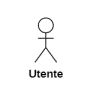
\includegraphics[scale = 1]{img/attori1.png}
L'utente generico, che potrà essere una persona fisica o anche un bot, potrà accedere a tutte le funzionalità del prodotto. \\
TODO aggiungere eventualmente come utenti il db di unsplash e servizi vari in futuro

\subsection{UC1 - Autenticazione}
\textbf{Attore primario}: Utente generico\\
\textbf{Precondizioni}: Il sistema non riconosce l'utente\\
\textbf{Postcondizioni}: L'utente è autenticato nel sistema\\

\textbf{Scenario principale}: L'utente:
	Inserisce il proprio username [UC1.1]

	Inserisce la propria password [UC1.2]

	Compila correttamente il captcha visualizzato [UC1.3]

\textbf{Scenari alternativi}:
\begin{enumerate}
    \item L'utente inserisce delle credenziali errate, il sistema mostra un errore e fa ritentare l'autenticazione all'utente. [UC4]
    \item L'utente non supera il captcha [uc”2”]: //da modificare UC3 diventa estensione di UC2
    \begin{enumerate}
	\item Nel caso in cui l'utente non abbia raggiunto il numero di tentativi massimo [UC2]:
	\begin{enumerate}
	    \item Viene visualizzato un errore esplicativo
	    \item L'utente non viene autenticato nel sistema
	    \item Il sistema fa ritentare l'autenticazione all'utente 
        \end{enumerate}
	\item Nel caso in cui l'utente abbia superato il numero di tentativi consentito per il superamento del captcha negli ultimi 20 minuti [UC3]:
	\begin{enumerate}
	    \item L'utente visualizza un messaggio di blocco
	    \item L'utente non viene autenticato nel sistema
	    \item Il sistema bloccherà futuri tentativi di autenticazione da parte di quell'utente per un tempo prestabilito
        \end{enumerate}
    \end{enumerate}
\end{enumerate}

\subsubsection{UC1.1 - Inserimento username}
\textbf{Attore primario}: Utente generico\\
\textbf{Precondizioni}: Il sistema non riconosce l'utente e non conosce l'username\\
\textbf{Postcondizioni}: Il sistema ha ricevuto l'username dell'utente\\
\textbf{Scenario principale}:
\begin{enumerate}
   \item L'utente inserisce l'username nell'apposito spazio. L'username deve essere quello preimpostato.
\end{enumerate}

\subsubsection{UC1.2 - Inserimento password}
\textbf{Attore primario}: Utente generico\\
\textbf{Precondizioni}: Il sistema non riconosce l'utente e non conosce la password\\
\textbf{Postcondizioni}: Il sistema ha ricevuto la password dell'utente\\
\textbf{Scenario principale}:
\begin{enumerate}
   \item L'utente inserisce la password nell'apposito spazio. L'username deve essere quello preimpostato.
\end{enumerate}

\subsubsection{UC1.3 - Compilazione captcha}
\textbf{Attore primario}: Utente generico\\
\textbf{Precondizioni}: L'utente visualizza il captcha proposto dal sistema\\
\textbf{Postcondizioni}: L'utente ha risolto il captcha (non necessariamente in modo corretto)\\
\textbf{Scenario principale}:
\begin{enumerate}
   \item L'utente risolve il captcha proposto, non necessariamente in maniera corretta
\end{enumerate}
\textbf{Generalizzazioni}:
\begin{itemize}
   \item captcha tipo 1 [UC1.3.1]
   \item captcha tipo 2 [UC1.3.2]
   \item ...
\end{itemize}

\paragraph{UC1.3.1 - Compilazione captcha tipo 1 (chiedere quanto si può andare in dettaglio)}~\smallskip
\textbf{Attore primario}: utente generico\\
\textbf{Precondizioni}: l'utente visualizza il captcha tipo 1\\
\textbf{Postcondizioni}: l'utente ha completato il captcha\\
\textbf{Scenario principale}:

All'utente viene presentato il captcha tipo 1, con 9 immagini da classificare
L'utente classifica le 9 immagini nelle giuste categorie


\paragraph{UC1.3.2 - Compilazione captcha tipo 2 [in realtà non esiste, serve solo per dire che siamo bravi e abbiamo previsto la generalizzazione per una futura estensione del sistema, capire dove scrivere questa cosa]}~\smallskip
\textbf{Attore primario}: utente generico\\
\textbf{Precondizioni}: l'utente visualizza il captcha tipo 2\\
\textbf{Postcondizioni}: l'utente ha completato il captcha\\
\textbf{Scenario principale}:

All'utente viene presentato il captcha tipo 2
[elenco delle azioni che servono per superare il captcha]

\subsection{UC2 - Captcha non superato}
\textbf{Attore primario}: Utente generico\\
\textbf{Precondizioni}: L'utente non ha compilato il captcha correttamente\\
\textbf{Postcondizioni}:L'utente visualizza un messaggio di errore e l'operazione di autenticazione fallisce. L'utente potrà riprovare ad autenticarsi\\
\textbf{Scenario principale}:
\begin{enumerate}
   \item L'utente visualizza un messaggio di errore
   \item Il numero di tentativi compiuti dall'utente negli ultimi 20 minuti aumenta di 1
   \item L'operazione di autenticazione fallisce
   \item Viene generato un altro captcha e l'utente potrà riprovare ad autenticarsi
\end{enumerate}

\subsection{UC3 - Superamento del numero di tentativi consentito}
\textbf{Attore primario}: Utente generico\\
\textbf{Precondizioni}: L'utente ha superato il numero massimo di tentativi di autenticazione consentiti e non ha compilato l'ultimo captcha correttamente\\
\textbf{Postcondizioni}:L'operazione di autenticazione fallisce e l'utente viene bloccato\\
\textbf{Scenario principale}:
\begin{enumerate}
   \item L'utente visualizza un messaggio di errore che comunica lo stato di blocco
   \item L'utente conferma di aver visualizzato il messaggio di errore
   \item L'operazione di autenticazione fallisce
   \item L'utente viene bloccato da futuri tentativi di login per un tempo prestabilito
\end{enumerate}

\subsection{UC4 - Credenziali errate}
\textbf{Attore primario}: Utente generico\\
\textbf{Precondizioni}:L'utente non ha inserito le credenziali corrette\\
\textbf{Postcondizioni}:L'utente visualizza un messaggio di errore e l'operazione di autenticazione fallisce. L'utente potrà riprovare  ad autenticarsi\\
\textbf{Scenario principale}:
\begin{enumerate}
   \item L'utente visualizza un messaggio di errore
   \item L'operazione di autenticazione fallisce
   \item Viene generato un altro captcha e l'utente potrà riprovare ad autenticarsi
\end{enumerate}

\subsection{UC5 - Generazione di un altro captcha (da chiedere su una possibile generalizzazione)}
\textbf{Attore primario}: Utente generico\\
\textbf{Precondizioni}: L'utente ha visualizzato il captcha proposto\\
\textbf{Postcondizioni}: All'utente viene proposto un nuovo captcha\\
\textbf{Scenario principale}:
\begin{enumerate}
   \item L'utente richiede la generazione di un nuovo captcha
   \item Il sistema propone all'utente un altro captcha
\end{enumerate}